\documentclass[6pt]{AiTex}
\usepackage{csvsimple}

\title{Memoria entrega 2}
\author{A.L.K.}
\date{Febrero 2024}

\begin{document}
%\datos{facultad}{universidad}{grado}{asignatura}{subtitulo}{autor}{curso}
\datos{Informática}{Universidad Complutense de Madrid}{Ingeniería informática}{Aprendizaje Automatico y Big Data}{Entrega 3: regresión lógica}{Alejandro Barrachina Argudo}{2023-2024}
% \portadaApuntes
% \pagestyle{empty}
% \tableofcontents
% \pagestyle{empty}
\justify

\begin{center}

    {\huge \textbf{\underline{\subtitulo}}} \\
    { \lesson - \autor}

\end{center}


\section*{Introducción}

En este documento se explicará el código del entregable 3 y el proceso de la regresión lógica. Esta práctica se divide en 2 apartados: regresión lógica y regresión lógica regularizada. Para ambos apartados se usan \textit{datasets}, el primero siendo un listado de notas de dos exámenes distintos de estudiantes y el otro resultado de tests de QA hechos a distintos chips para comprobar si son válidos o no.

Para esta práctica se usarán los siguientes \textit{imports} vistos en la figura \ref{fig:imports}.

\begin{figure}[H]
    \centering
    \lstinputlisting[firstline=1,lastline=5, style=custompython]{../logistic_reg.py}
    \caption{Código de las bibliotecas usadas}
    \label{fig:imports}
\end{figure}

También se usarán los siguientes strings estáticos durante toda la ejecución del programa (figura \ref{fig:strings}).

\begin{figure}[H]
    \centering
    \lstinputlisting[firstline=7,lastline=9, style=custompython]{../logistic_reg.py}
    \caption{Código de los strings estáticos}
    \label{fig:strings}
\end{figure}

\section{Parte A: Regresión lógica}

En esta parte haremos una regresión lógica simple sobre el primer dataset para predecir si un estudiante va a pasar la asignatura en base a sus dos primeras notas (distribución visible en la figura \ref{fig:dataset1}). Para ello usaremos la función $f_{w,b}(x^{(i)} = g(w * x^{(i)} +b))$ (implementación en la figura \ref{fig:function}), siendo $g$ el sigmoide implementado en la función \textit{sigmoid} (figura \ref{fig:sigmoid}).

Para seguir con el aprendizaje del modelo tendremos que implementar las funciones de coste y de gradiente, que se implementan en las figuras \ref{fig:cost} y \ref{fig:grad} respectivamente. La función de coste se expresa como \[J(w,b) = \frac{1}{m} \sum_{i=0}^{m -1} [loss(f_{w,b}(x^{(i)}),y^{(i)})]\] siendo $loss$ la función de pérdida que se implementa en la figura \ref{fig:loss} y cuya fórmula matemática es \[loss(f_{w,b}(x^{i}), y^{i}) = (-y^{(i)}log(f_{w,b}(x^{i})) - (1-y^{i})log(1-f_{w,b}(x^{i})))\]

La función de gradiente tiene dos partes, una para $w$ y otra para $b$, cuya fórmula matemática se representa como \[\frac{\partial J(w,b)}{\partial w} = \frac{1}{m} \sum_{i=1}^{m} x^{(i)} * (f_{w,b}(x^{(i)}) - y^{(i)})\] \[\frac{\partial J(w,b)}{\partial b} = \frac{1}{m} \sum_{i=1}^{m} (f_{w,b}(x^{(i)}) - y^{(i)})\] respectivamente.

Para estas funciones tenemos la opción de pasarle un argumento \textit{lambda} que por ahora solo estará ahí como placeholder para no interferir con las funciones del segundo apartado.

Para terminar esta parte. se implemente un descenso de gradiente (implementado en la figura \ref{fig:gradient_descent}) por número de iteraciones donde $w$ y $b$ se actualizan en cada iteración según la fórmula \[w = w - \alpha \frac{\partial J(w,b)}{\partial w}\] \[b = b - \alpha \frac{\partial J(w,b)}{\partial b}\] siendo $\alpha$ la tasa de aprendizaje. Siguiendo los valores del ejemplo dado en el enunciado ( $b = -8$, $\vec{w} = 0$ y $\alpha = 0.001$) se obtiene que $\vec{w} = [0.07125349, 0.06482881]$, y $b = -8.188614567810179$ con $J(w,b) = 0.3018682223181452$ tras 10000 iteraciones. Podemos ver la barrera de decisión en la figura \ref{fig:decision_boundary1}.

\begin{figure}[H]
    \centering
    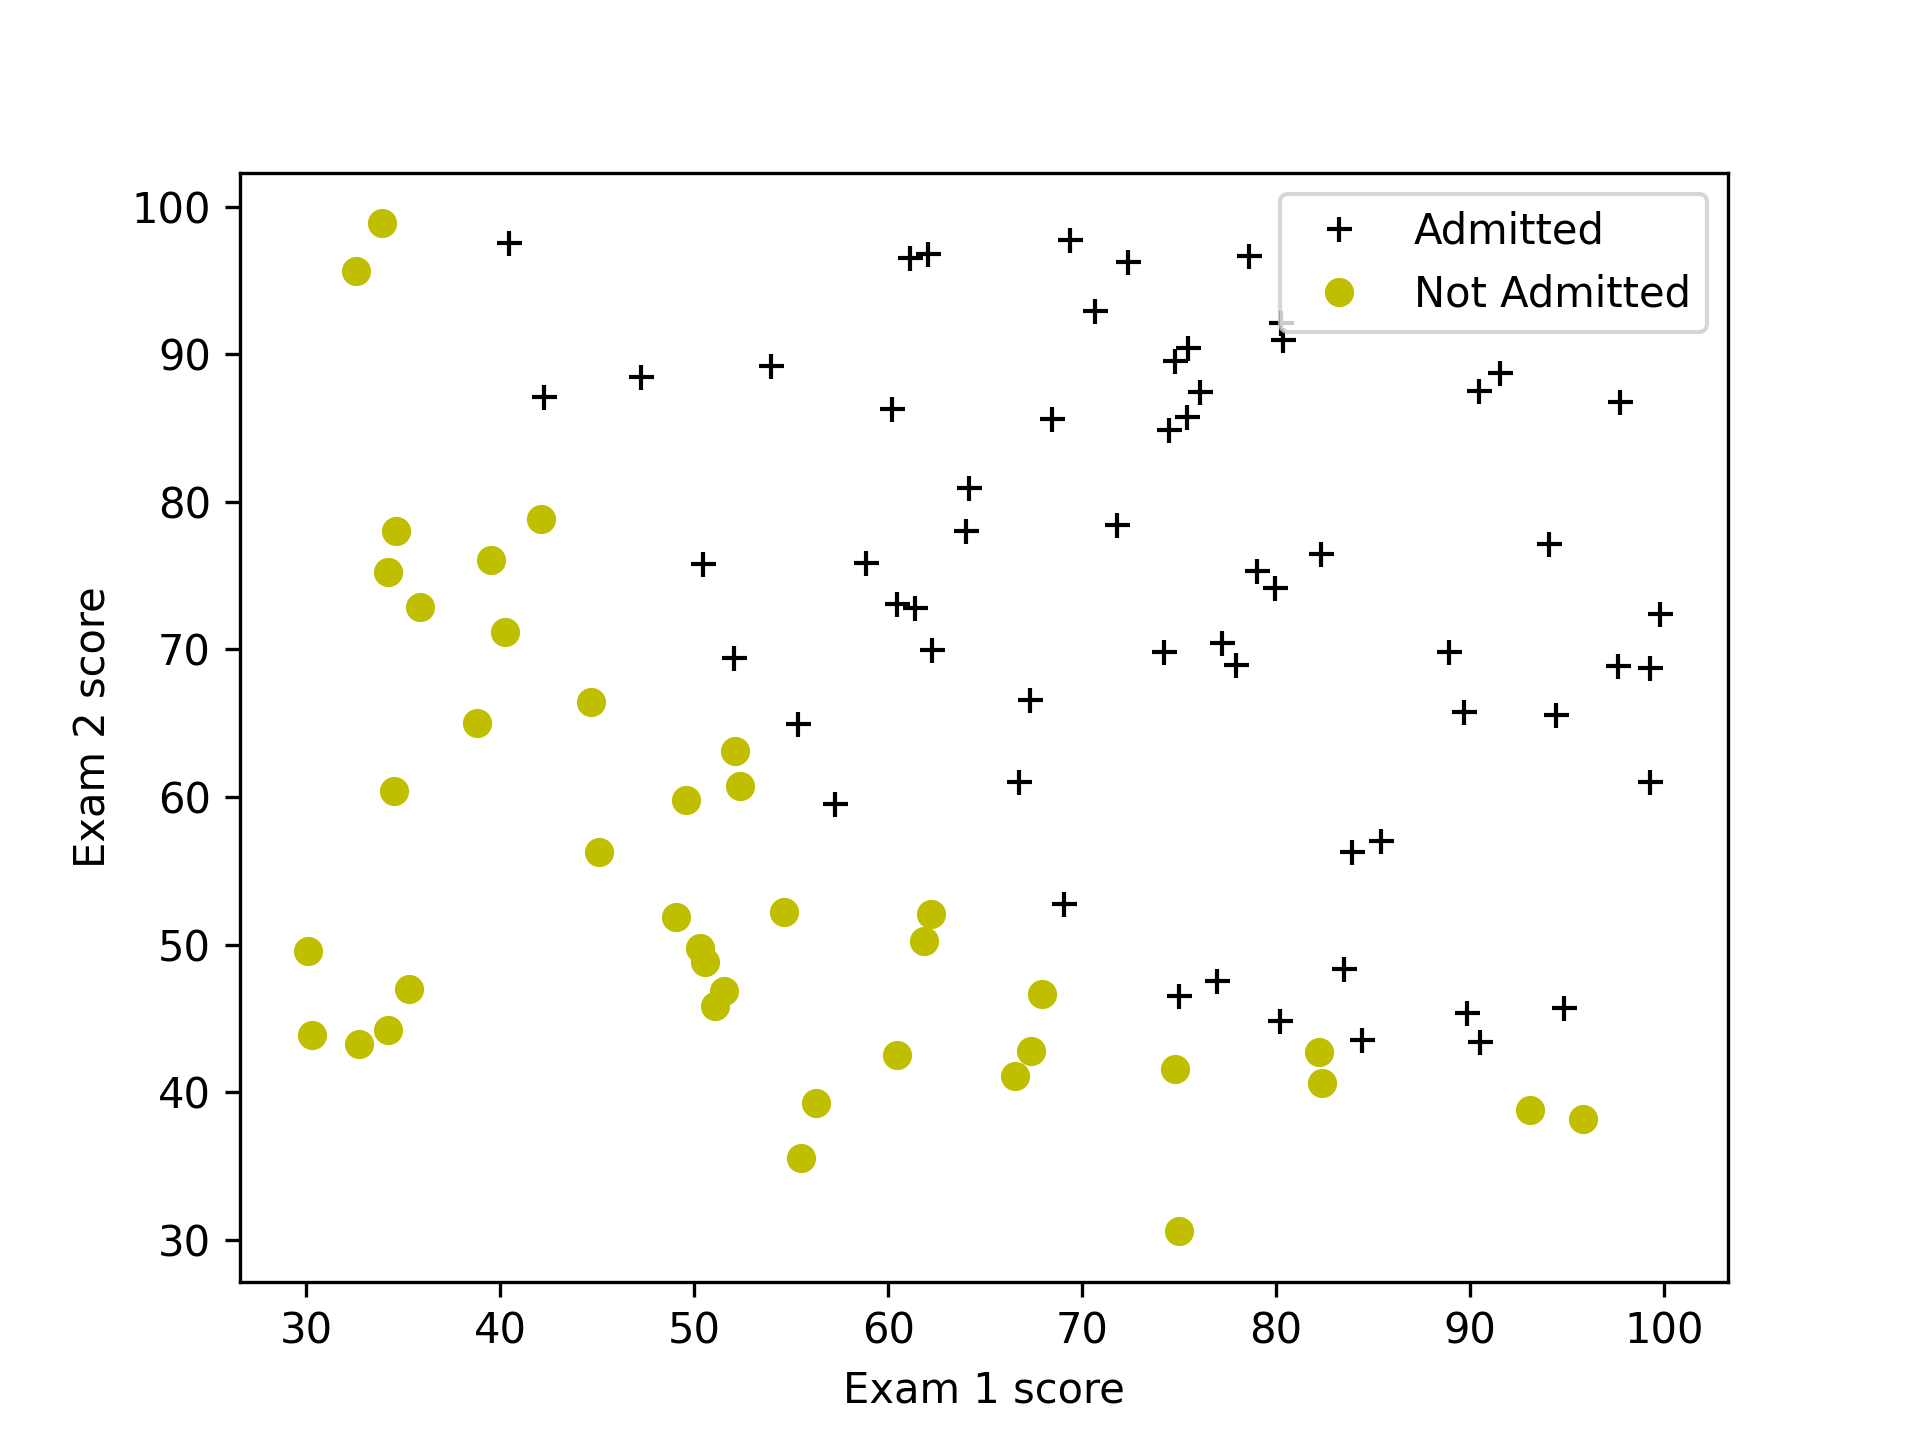
\includegraphics[width=0.5\textwidth]{./imagenes/muestreo1.png}
    \caption{Distribución de notas de estudiantes}
    \label{fig:dataset1}
\end{figure}

\begin{figure}[H]
    \centering
    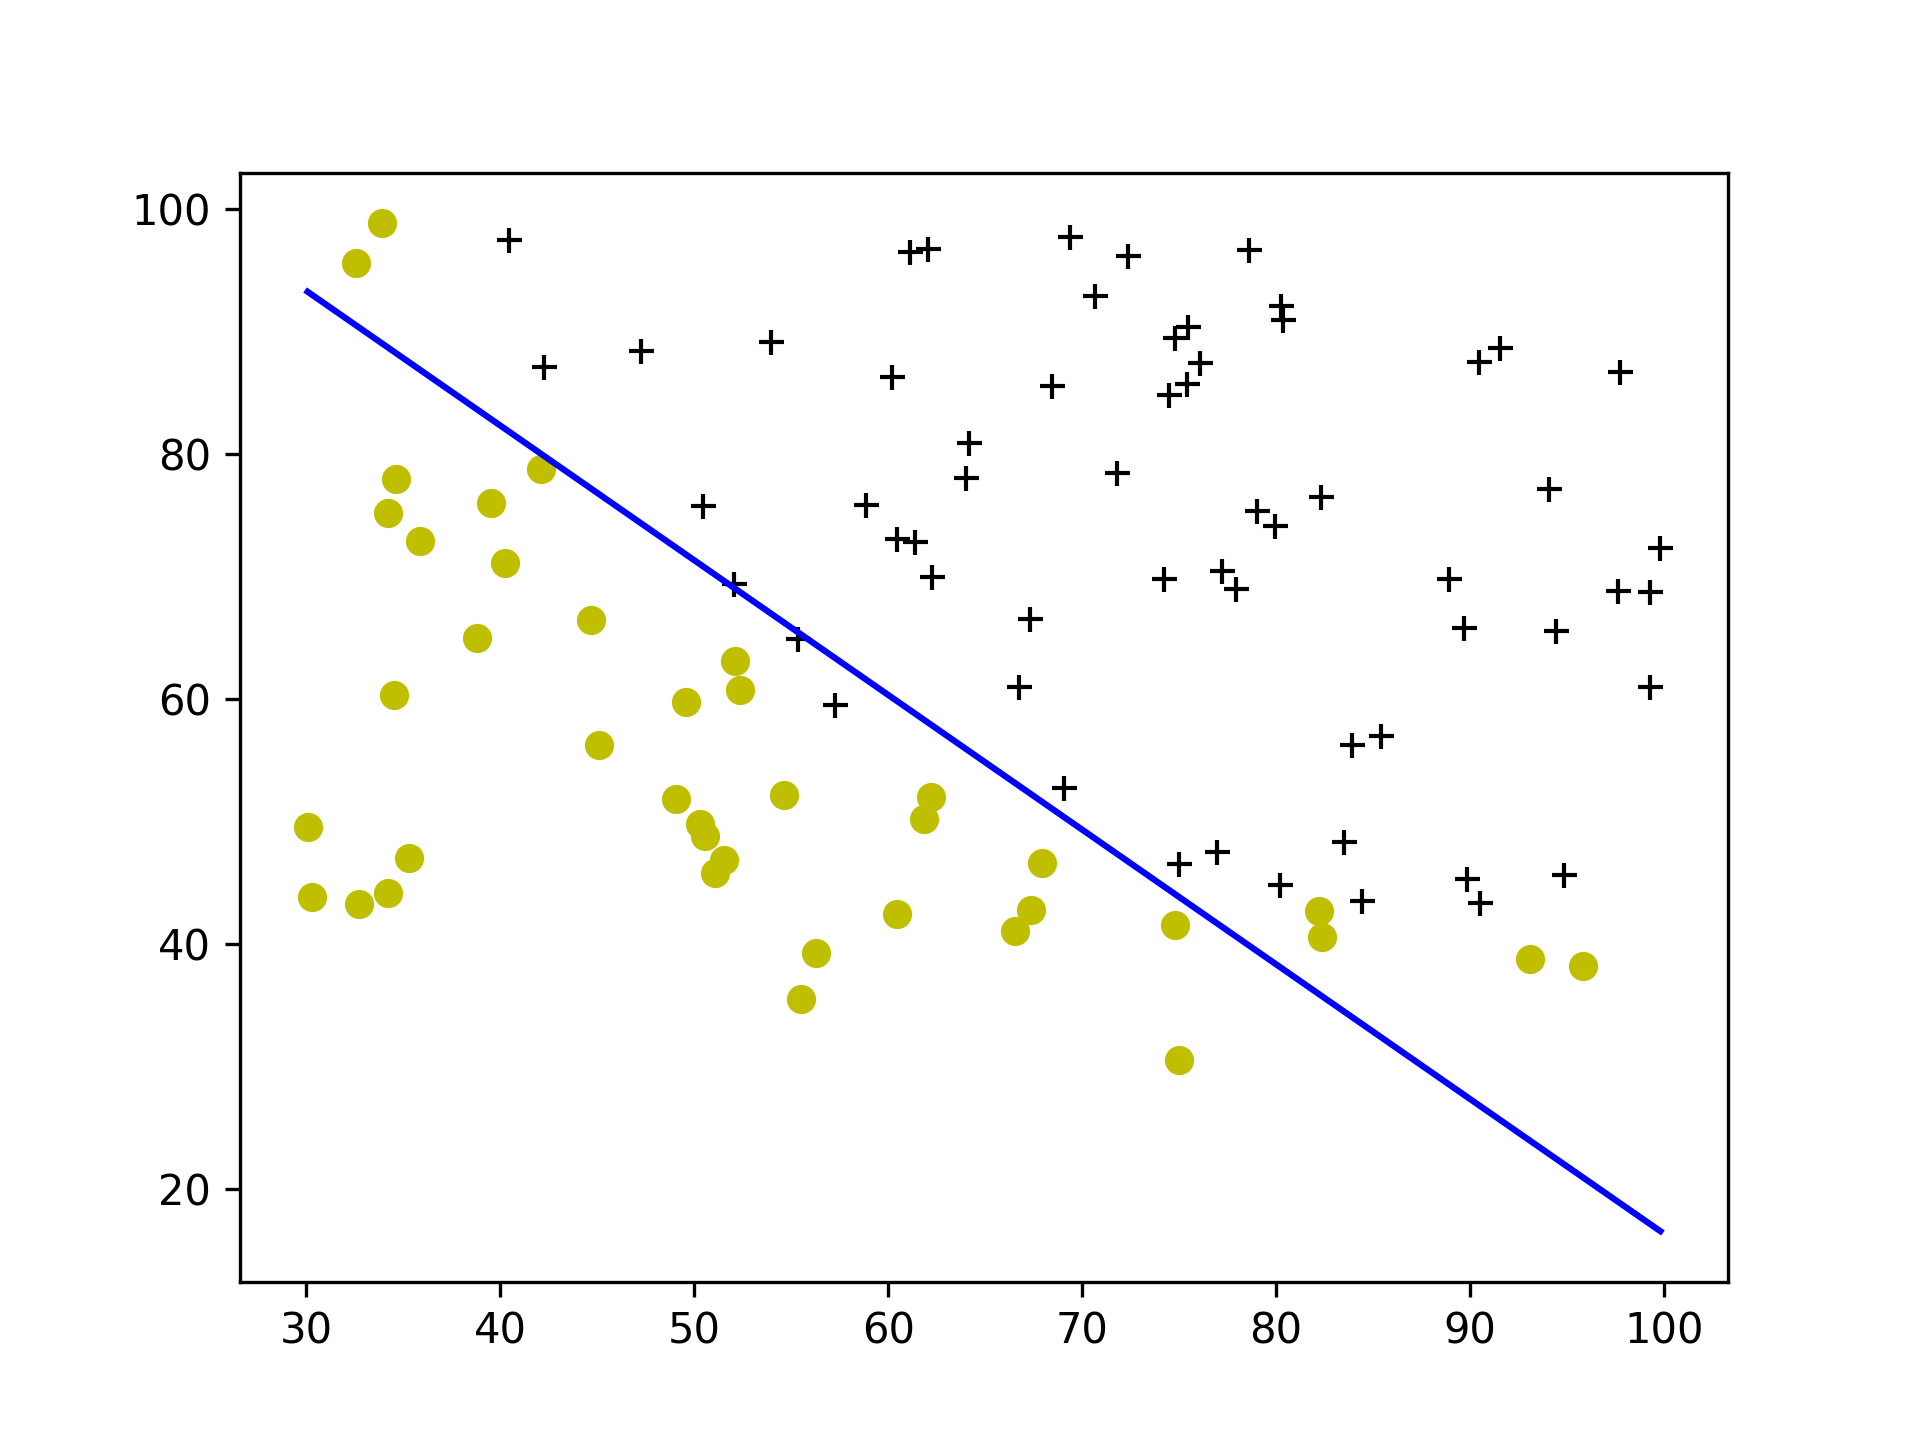
\includegraphics[width=0.5\textwidth]{./imagenes/muestreo1_sim.png}
    \caption{Barrera de decisión}
    \label{fig:decision_boundary1}
\end{figure}

\begin{figure}[H]
    \centering
    \lstinputlisting[firstline=32,lastline=43, style=custompython]{../logistic_reg.py}
    \caption{Función de regresión lógica}
    \label{fig:function}
\end{figure}

\begin{figure}[H]
    \centering
    \lstinputlisting[firstline=12,lastline=26, style=custompython]{../logistic_reg.py}
    \caption{Función sigmoide}
    \label{fig:sigmoid}
\end{figure}

\begin{figure}[H]
    \centering
    \lstinputlisting[firstline=62,lastline=79, style=custompython]{../logistic_reg.py}
    \caption{Función de coste}
    \label{fig:cost}
\end{figure}

\begin{figure}[H]
    \centering
    \lstinputlisting[firstline=46,lastline=59, style=custompython]{../logistic_reg.py}
    \caption{Función de perdida}
    \label{fig:loss}
\end{figure}

\begin{figure}[H]
    \centering
    \lstinputlisting[firstline=82,lastline=105, style=custompython]{../logistic_reg.py}
    \caption{Función de gradiente}
    \label{fig:grad}
\end{figure}

\begin{figure}[H]
    \centering
    \lstinputlisting[firstline=154,lastline=190, style=custompython]{../logistic_reg.py}
    \caption{Descenso de gradiente}
    \label{fig:gradient_descent}
\end{figure}

\section{Parte B: Regresión lógica regularizada}

En esta parte se implementa una regresión lógica regularizada para predecir si un chip va a ser valido basándonos en distintos datos de QA (distribución en la figura \ref{fig:dataset2}). Para este apartado seguiremos usando la función sigmoide implementada en la figura \ref{fig:sigmoid} y la función de regresión de la figura \ref{fig:function}. La función de coste y de gradiente se implementan en las figuras \ref{fig:cost_reg} y \ref{fig:grad_reg} respectivamente. La función de coste se expresa como \[J(w,b) = \frac{1}{m} \sum_{i=0}^{m -1} [loss(f_{w,b}(x^{(i)}),y^{(i)})] + \frac{\lambda}{2m} \sum_{j=1}^{n} w_j^2\] siendo $\lambda$ el parámetro de regularización y $n$ el número de características. La función de gradiente tiene dos partes, una para $w$ y otra para $b$, cuya fórmula matemática se representa como \[\frac{\partial J(w,b)}{\partial w} = \frac{1}{m} \sum_{i=1}^{m} x^{(i)} * (f_{w,b}(x^{(i)}) - y^{(i)}) + \frac{\lambda}{m} w\] \[\frac{\partial J(w,b)}{\partial b} = \frac{1}{m} \sum_{i=1}^{m} (f_{w,b}(x^{(i)}) - y^{(i)})\] respectivamente. Para este apartado usaremos el descenso de gradiente del apartado anterior (figura \ref{fig:gradient_descent}) dándole uso a la variable lambda\_.

Utilizando las métricas dadas en el enunciado ($b = 1$, $\vec{w} = 0$, $\lambda = 0.01$ y $\alpha = 0.01$), obtenemos $J(w,b) = 0.449111111581372$, $b = 1.3575493852806007$ y w:

\begin{table}[H]
    \centering
    \begin{tabular}{|c|}
        \hline
        \textbf{w}  \\
        \hline
        0.72259293  \\ \hline
        1.37503464  \\ \hline
        -2.26623624 \\ \hline
        -0.93538886 \\ \hline
        -1.43093541 \\ \hline
        0.10544778  \\ \hline
        -0.38027447 \\ \hline
        -0.38596694 \\ \hline
        -0.21958157 \\ \hline
        -1.67262795 \\ \hline
        -0.09567878 \\ \hline
        -0.65568869 \\ \hline
        -0.27805803 \\ \hline
        -1.34114809 \\ \hline
        -0.30618779 \\ \hline
        -0.23477687 \\ \hline
        -0.07613709 \\ \hline
        -0.29039658 \\ \hline
        -0.30685795 \\ \hline
        -0.6307361  \\ \hline
        -1.21790115 \\ \hline
        -0.00397421 \\ \hline
        -0.32015246 \\ \hline
        -0.00392708 \\ \hline
        -0.35180518 \\ \hline
        -0.14316118 \\ \hline
        -1.15539835 \\ \hline
    \end{tabular}
    \caption{Tabla de pesos}
    \label{tab:w}
\end{table}

Podemos ver la barrera de decisión en la figura \ref{fig:decision_boundary2}.

\begin{figure}[H]
    \centering
    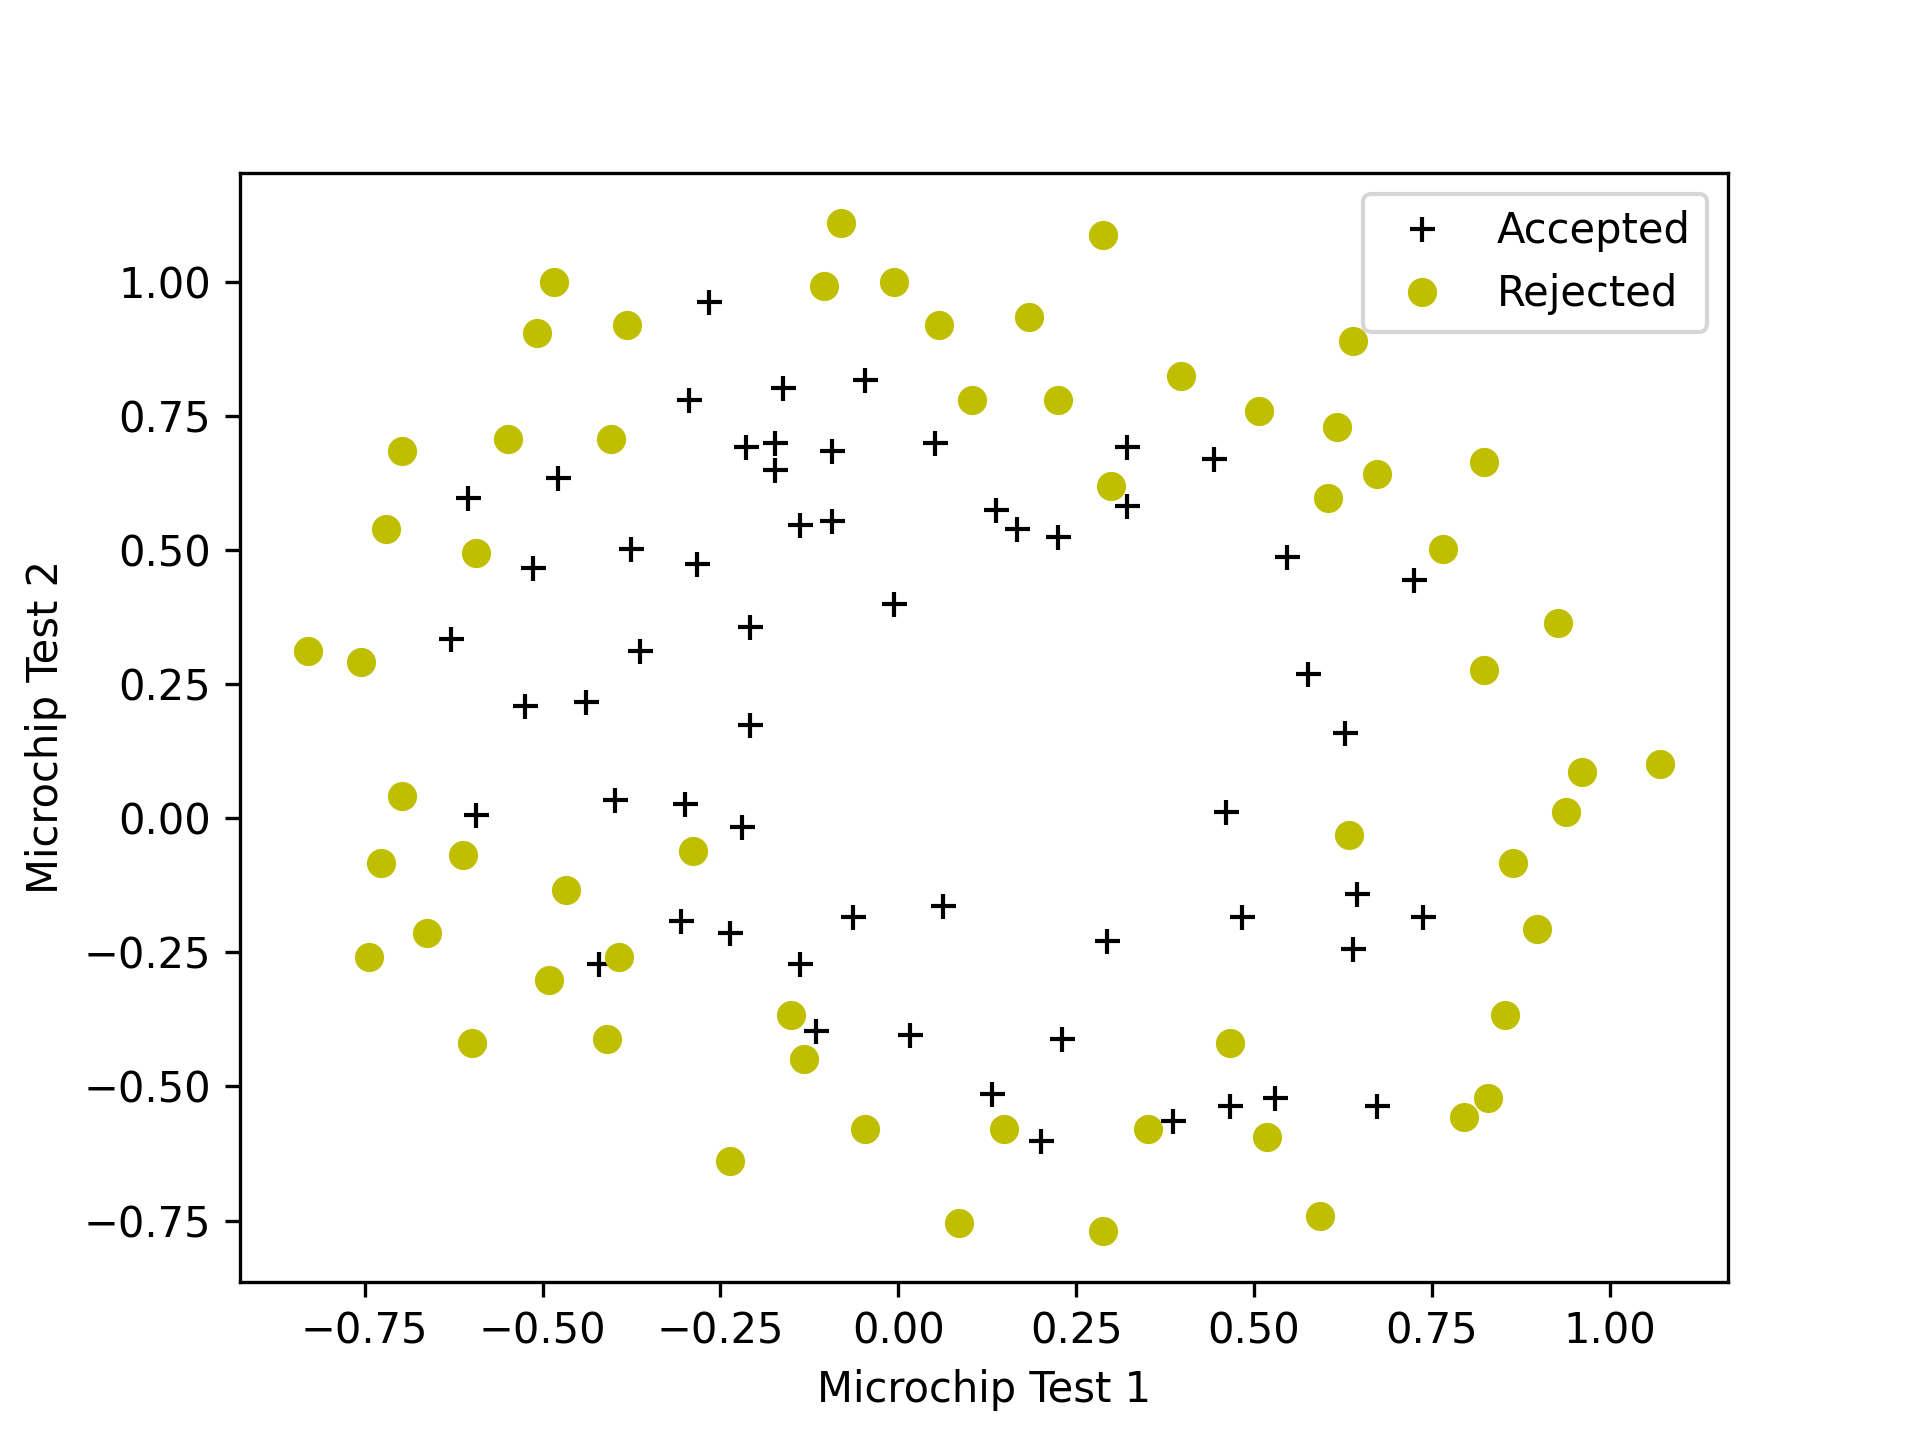
\includegraphics[width=0.5\textwidth]{./imagenes/muestreo2.png}
    \caption{Distribución de datos de QA de chips}
    \label{fig:dataset2}
\end{figure}

\begin{figure}[H]
    \centering
    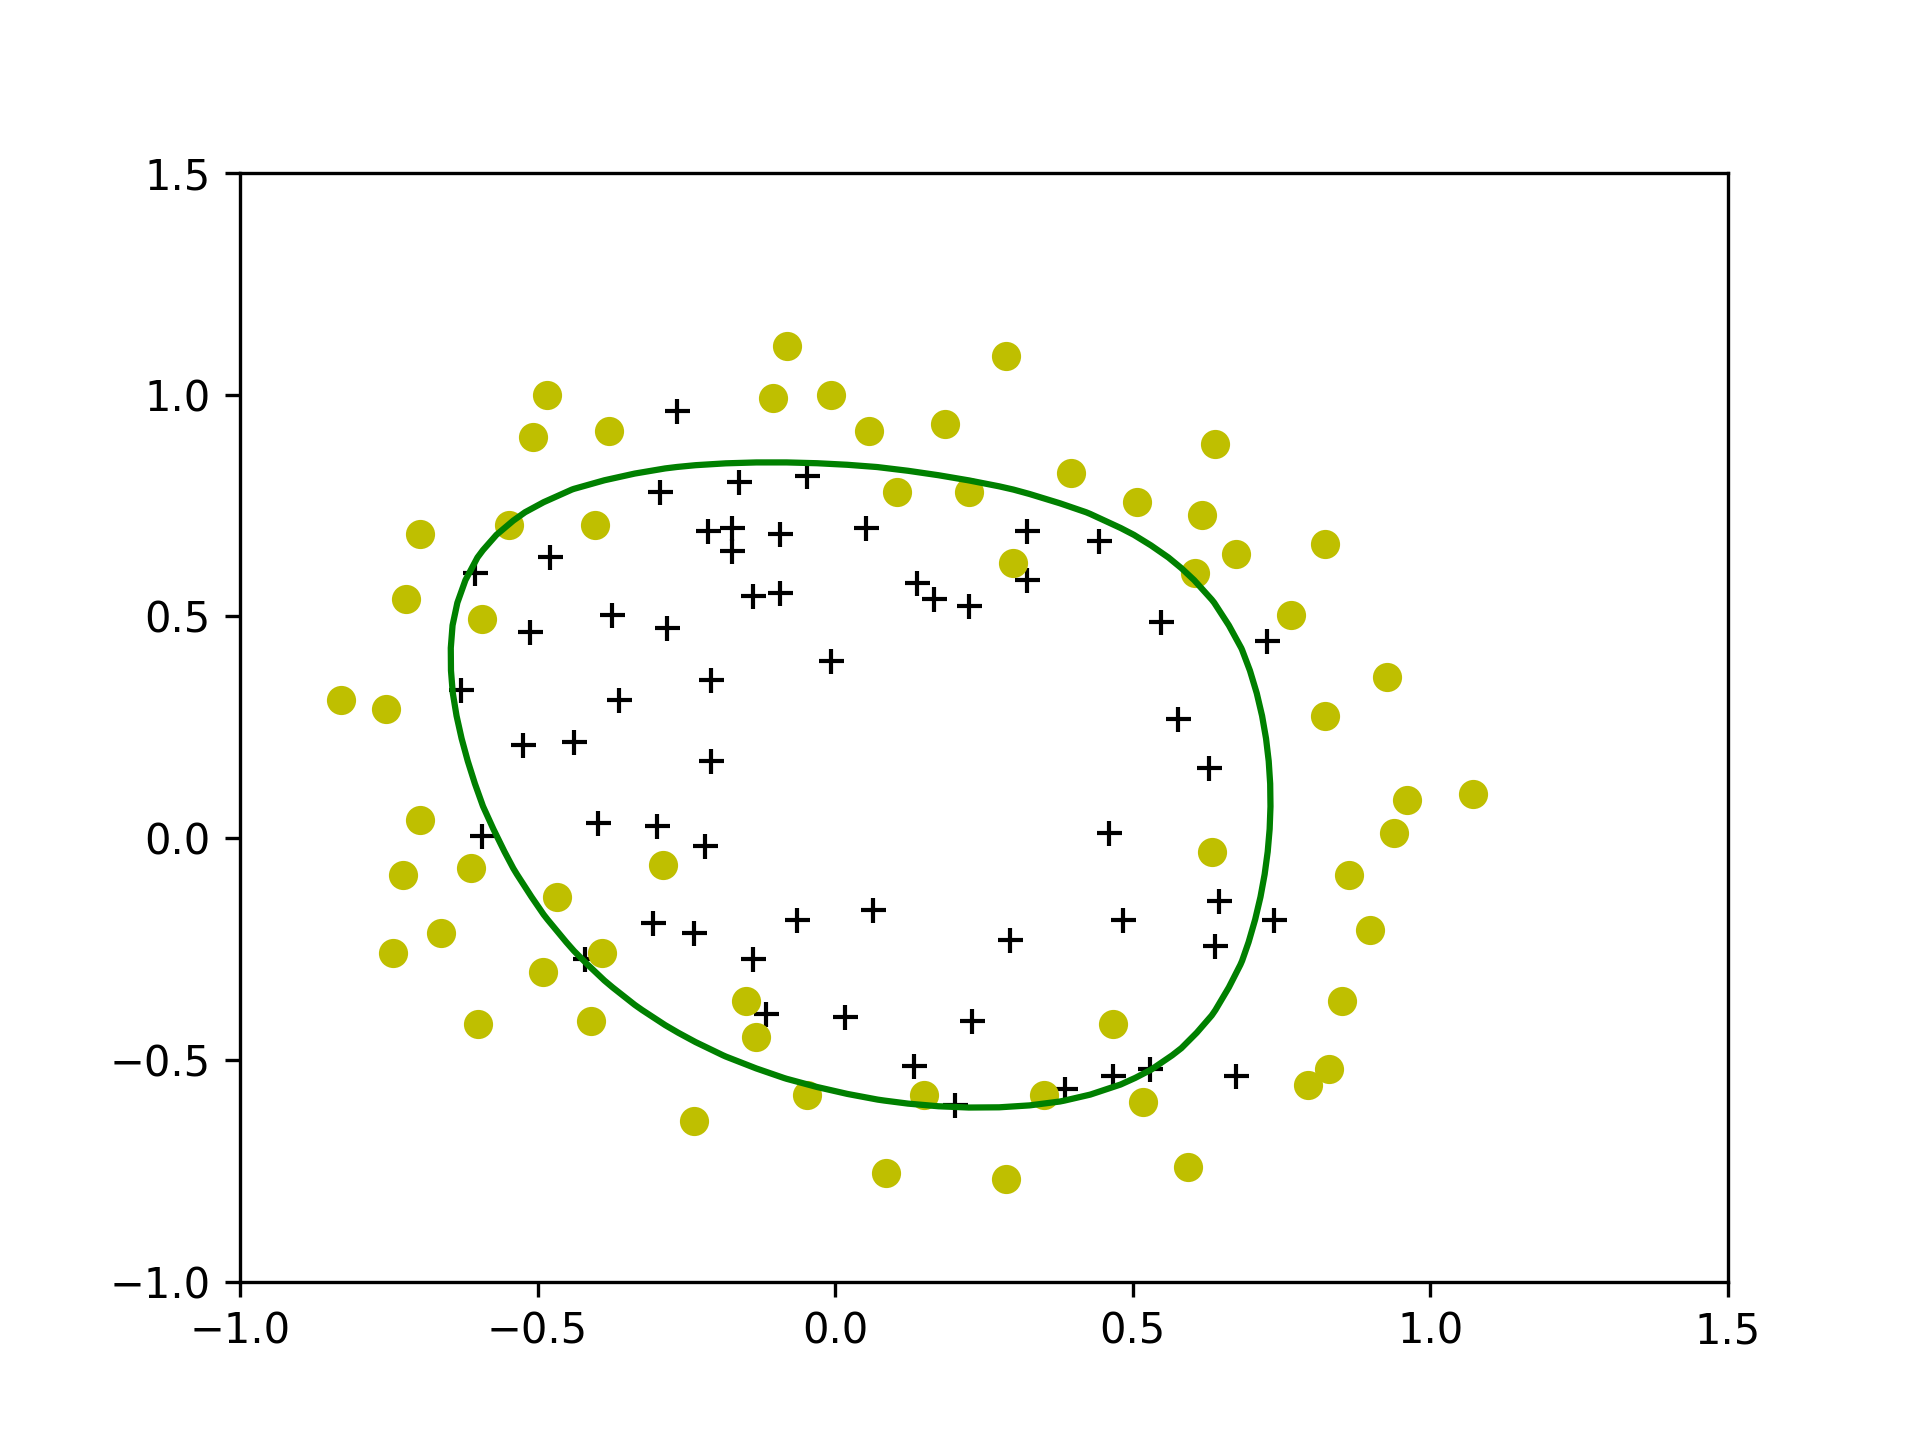
\includegraphics[width=0.5\textwidth]{./imagenes/muestreo2_sim.png}
    \caption{Barrera de decisión}
    \label{fig:decision_boundary2}
\end{figure}

\begin{figure}[H]
    \centering
    \lstinputlisting[firstline=111,lastline=127, style=custompython]{../logistic_reg.py}
    \caption{Función de coste regularizada}
    \label{fig:cost_reg}
\end{figure}

\begin{figure}[H]
    \centering
    \lstinputlisting[firstline=130,lastline=148, style=custompython]{../logistic_reg.py}
    \caption{Función de gradiente regularizada}
    \label{fig:grad_reg}
\end{figure}

\section{Predicciones, test de funciones y ejecución del programa}

Para comprobar estos modelos, hacemos una predicción de cada modelo con la función \textit{predict} (figura \ref{fig:predict}) y comprobamos su precisión con la función \textit{predict\_check} (figura \ref{fig:predict_check}). Para cargar todos los datos del dataset usamos la función \textit{load\_data} (figura \ref{fig:load_data}), y para ejecutar ambos modelos usamos las funciones \textit{run\_student\_sim} (figura \ref{fig:run_student_sim}) y \textit{run\_chip\_sim} (figura \ref{fig:run_chip_sim}).

Antes de ejecutar ambos modelos, se ejecutan las pruebas para ver que todo funciona usando la función \textit{run\_tests} (figura \ref{fig:run_tests}). Para visualizar mejor los datos usaremos la función \textit{plot\_ex\_data} (figura \ref{fig:plot_ex_data}) para los datos de ejemplo y \textit{plot\_linear\_data} (figura \ref{fig:plot_linear_data}) para la evolución del coste y de la predicción en cada iteración.

Tras las ejecuciones de ambas simulaciones, obtenemos un porcentaje de acierto del $92\%$ en el primer modelo y un $83.05084745762711\%$ en el segundo y podemos ver las siguientes gráficas:
\begin{itemize}
    \item Evolución del coste (figura \ref{fig:cost_evolution1}) y de la predicción (figura \ref{fig:prediction_evolution1}) para el primer dataset.
    \item Evolución del coste (figura \ref{fig:cost_evolution2}) y de la predicción (figura \ref{fig:prediction_evolution2}) para el segundo dataset.
\end{itemize}

\begin{figure}[H]
    \centering
    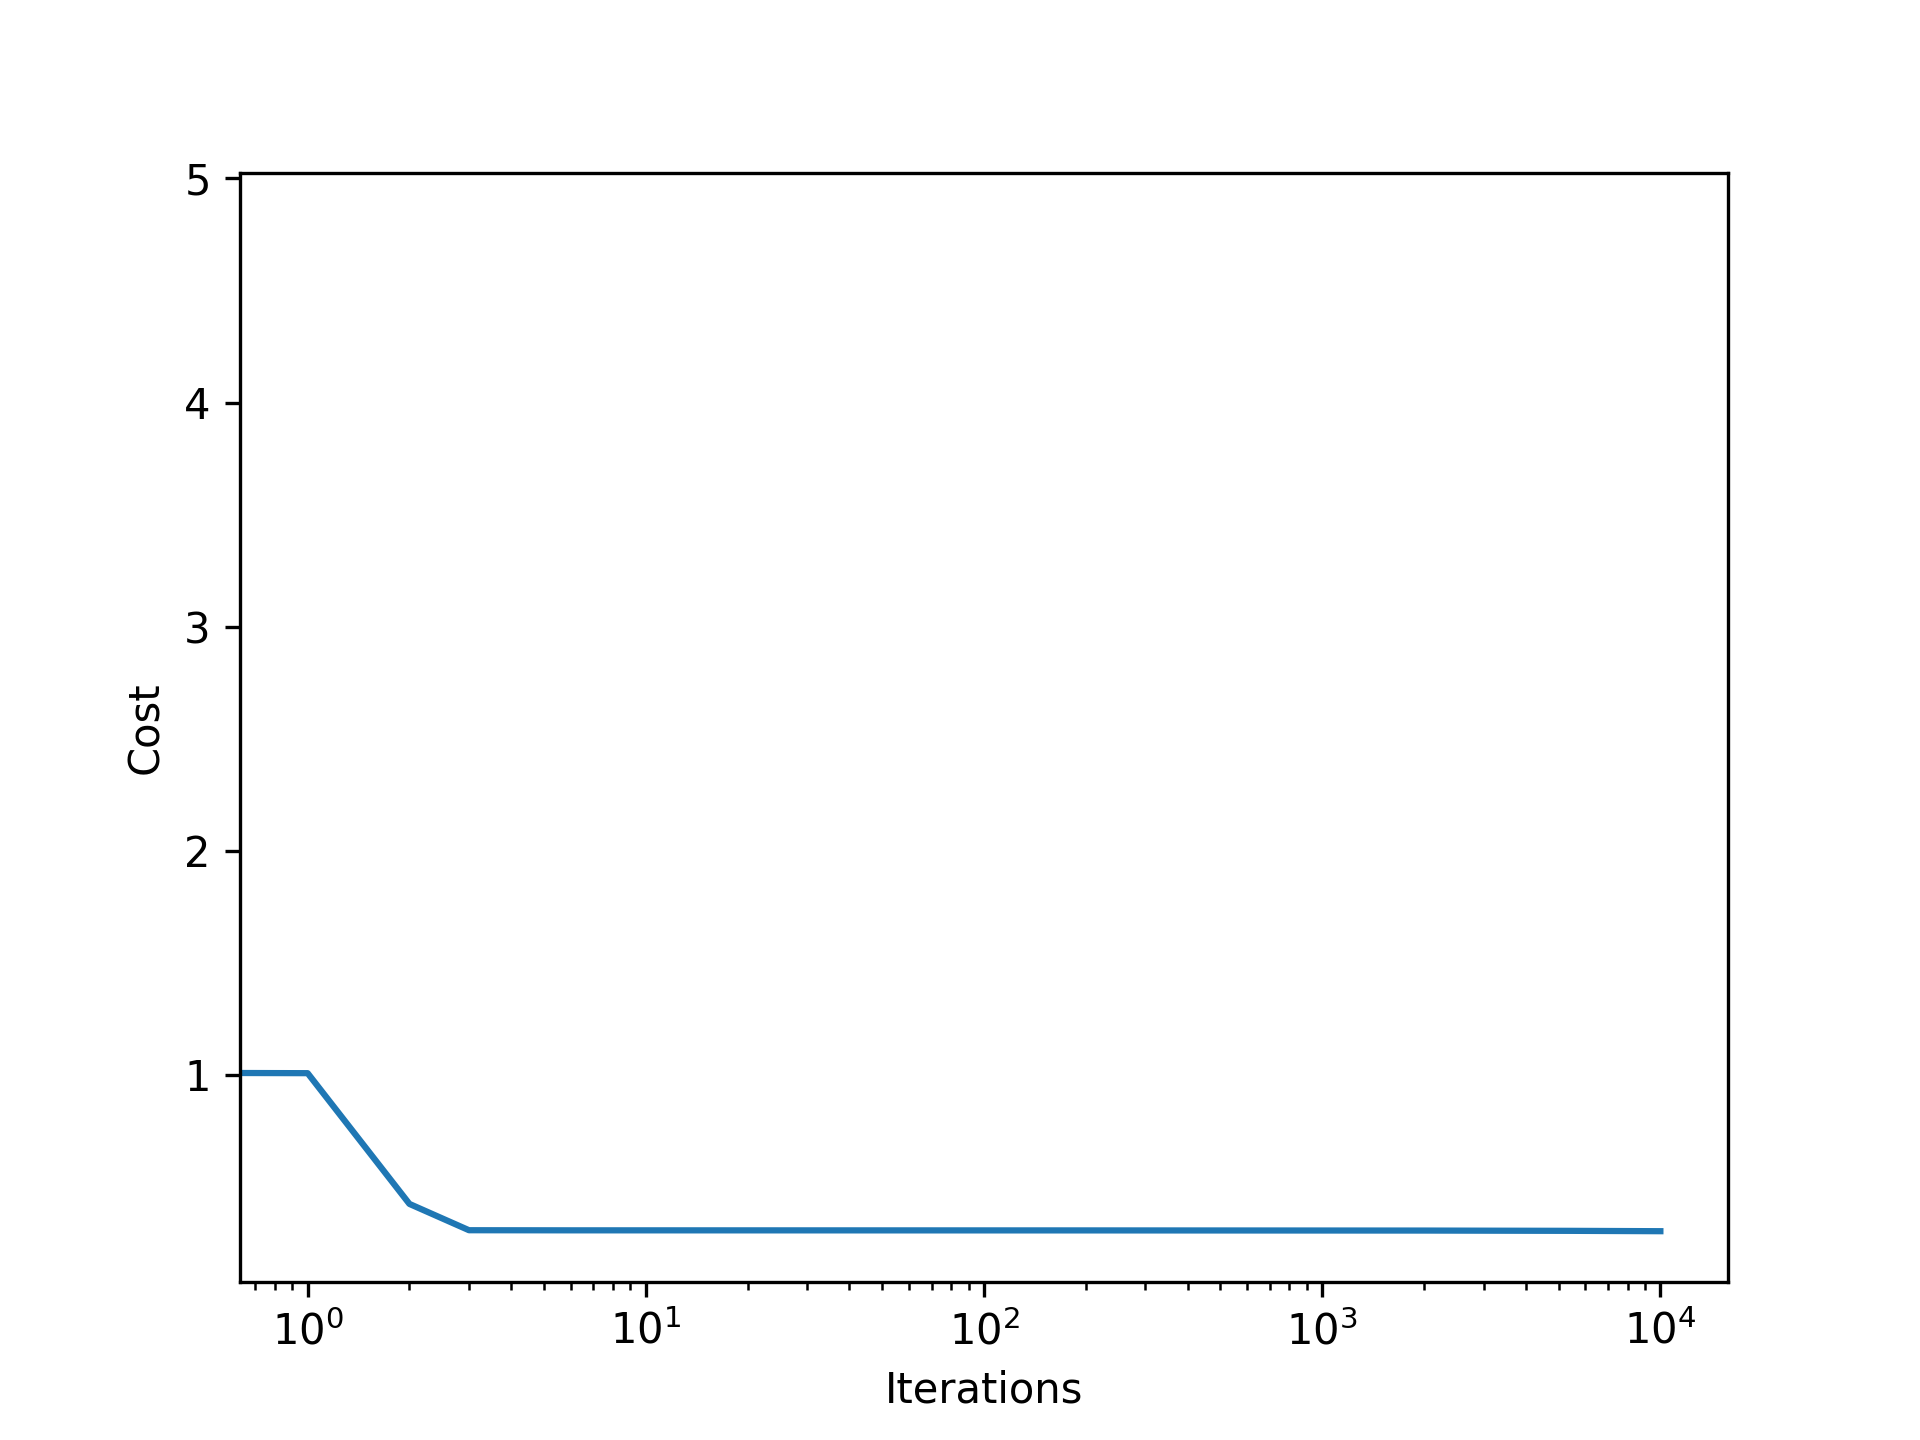
\includegraphics[width=0.5\textwidth]{./imagenes/muestreo1_cost.png}
    \caption{Evolución del coste para el primer dataset}
    \label{fig:cost_evolution1}
\end{figure}

\begin{figure}[H]
    \centering
    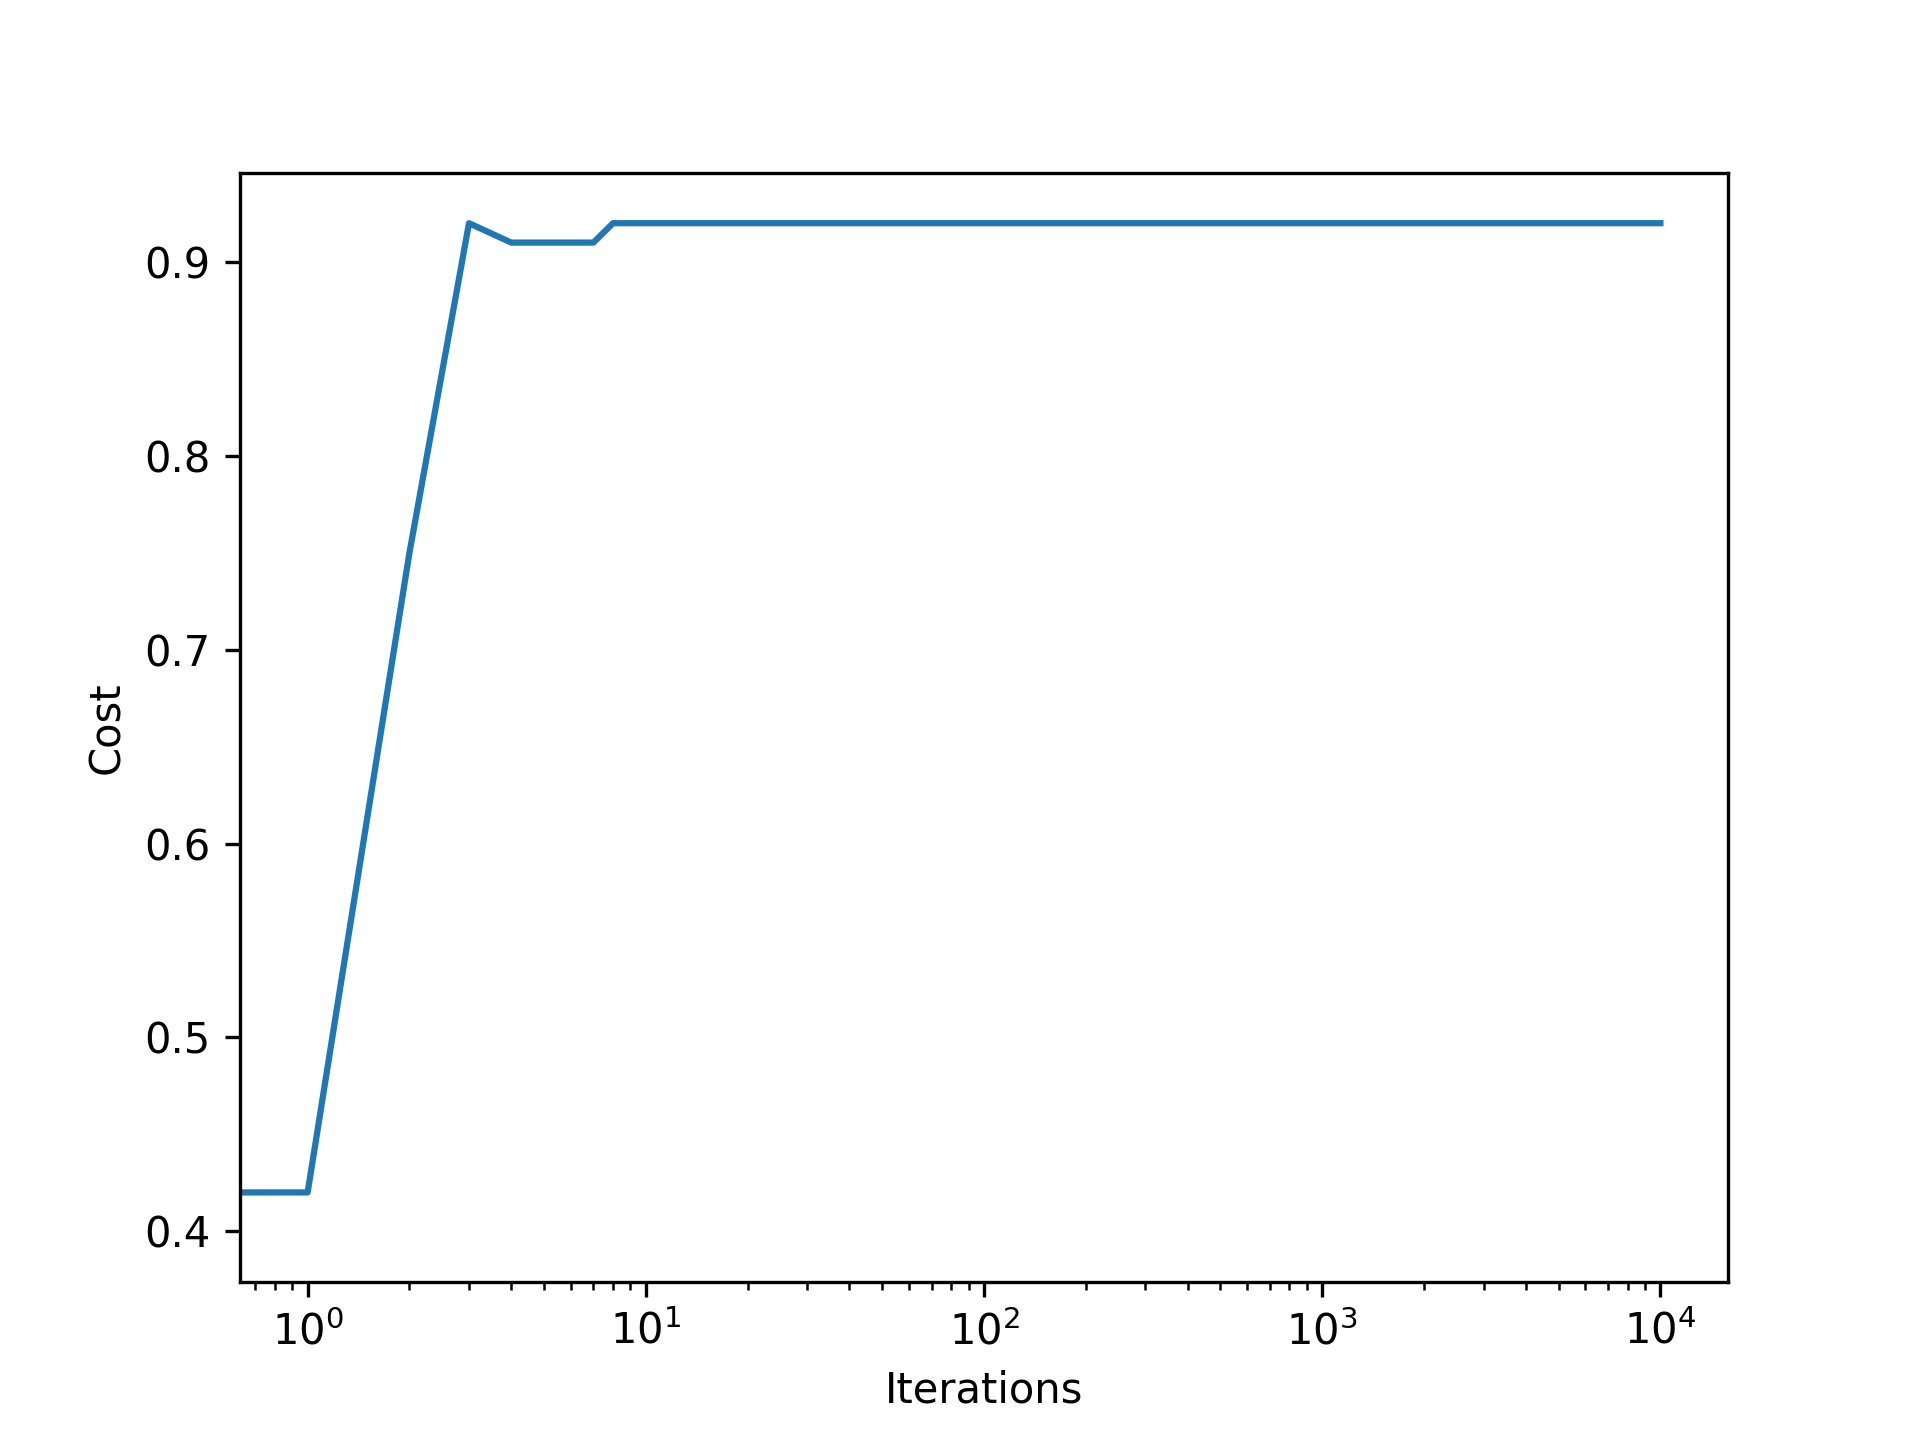
\includegraphics[width=0.5\textwidth]{./imagenes/muestreo1_accuracy.png}
    \caption{Evolución de la predicción para el primer dataset}
    \label{fig:prediction_evolution1}
\end{figure}

\begin{figure}[H]
    \centering
    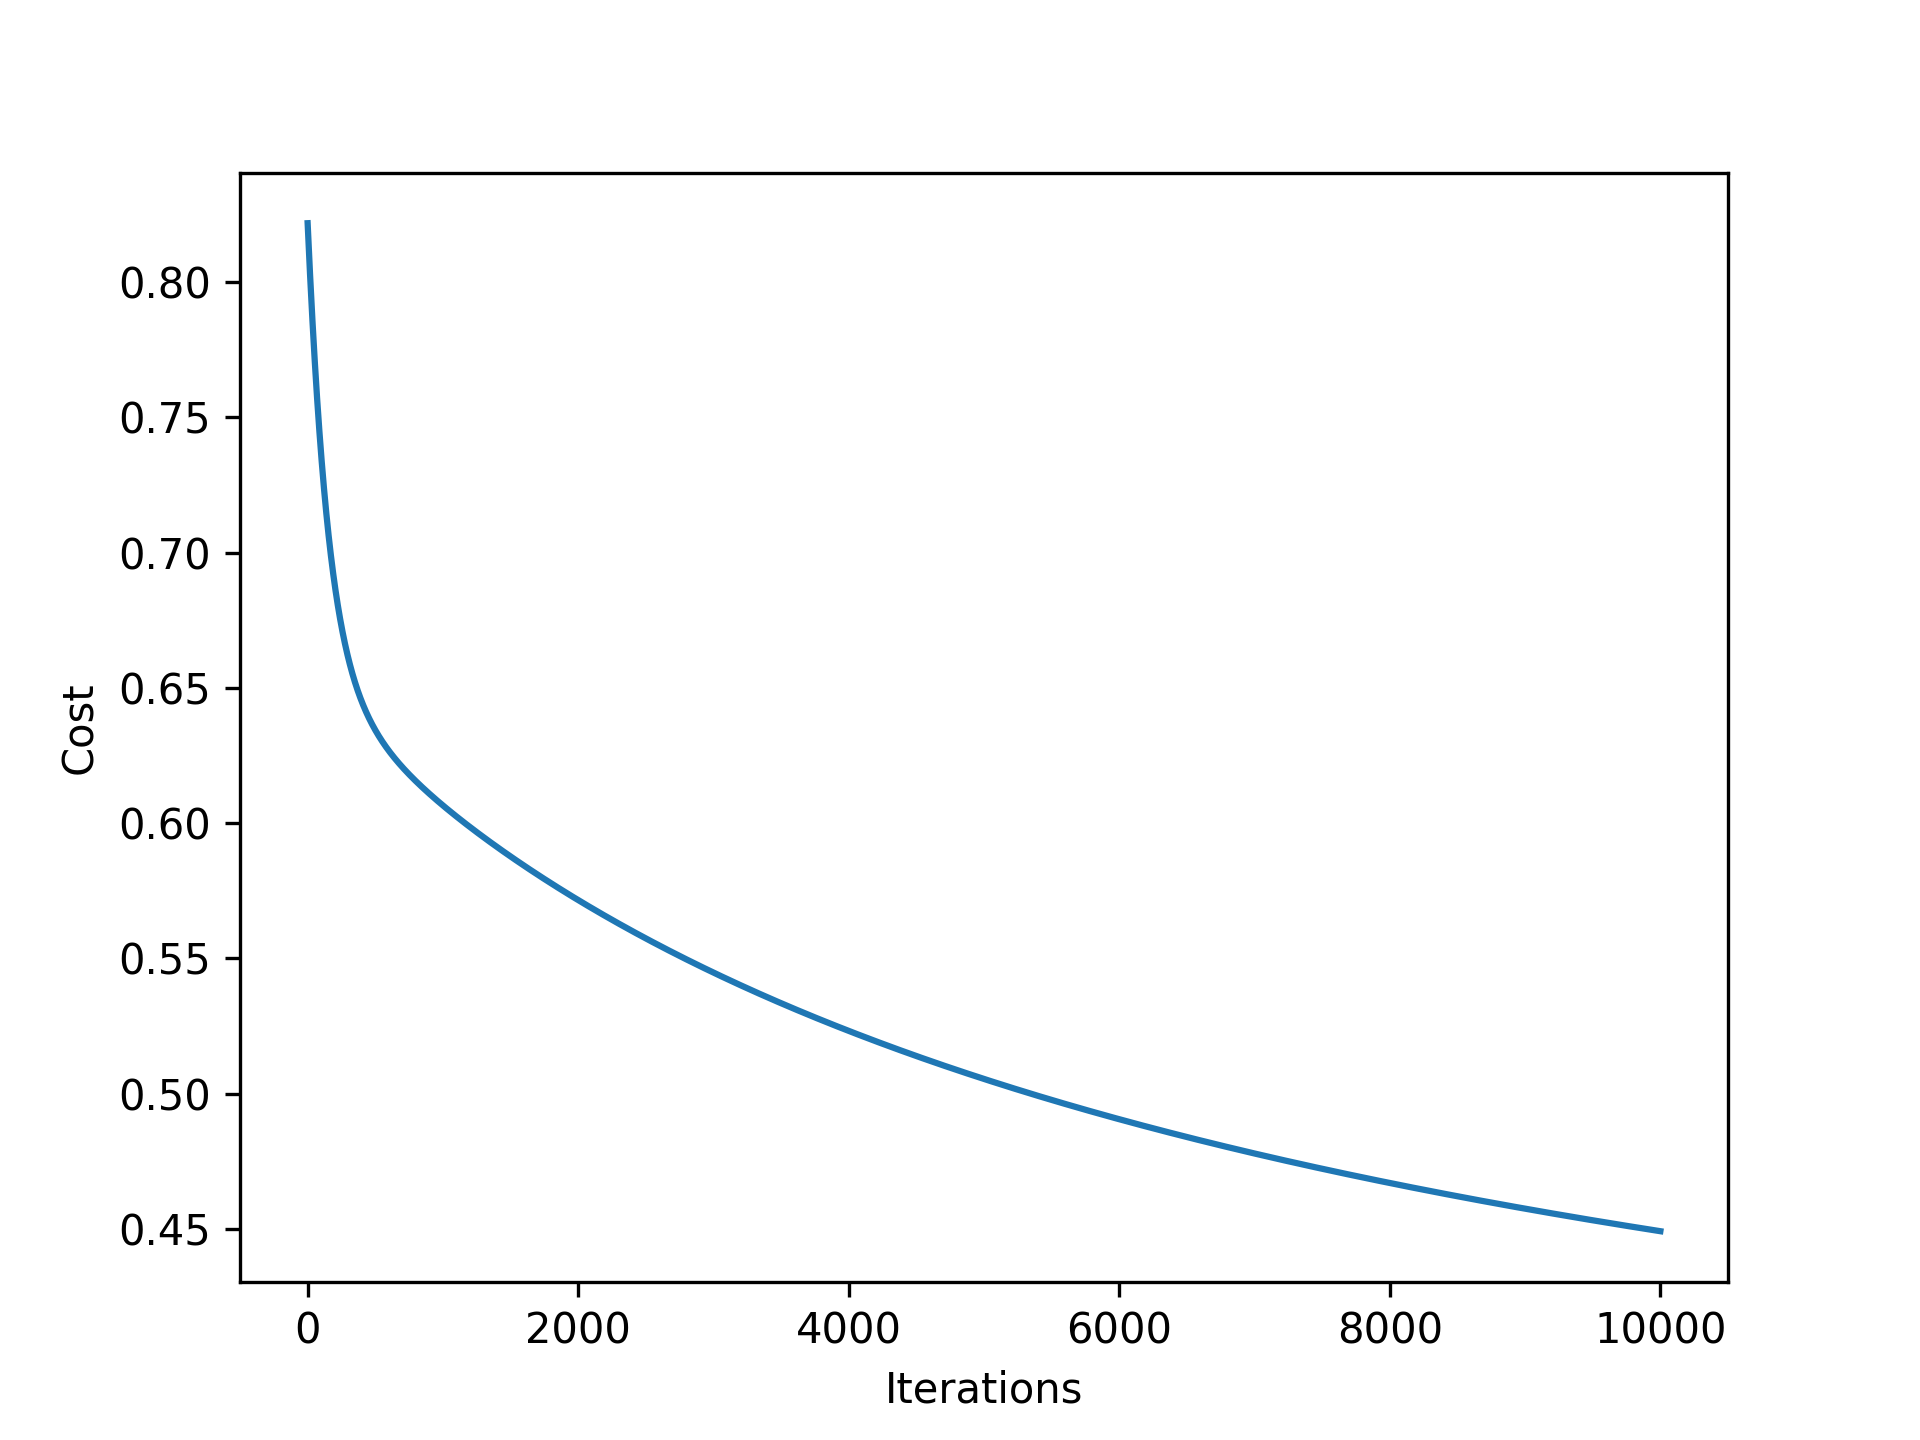
\includegraphics[width=0.5\textwidth]{./imagenes/muestreo2_cost.png}
    \caption{Evolución del coste para el segundo dataset}
    \label{fig:cost_evolution2}
\end{figure}

\begin{figure}[H]
    \centering
    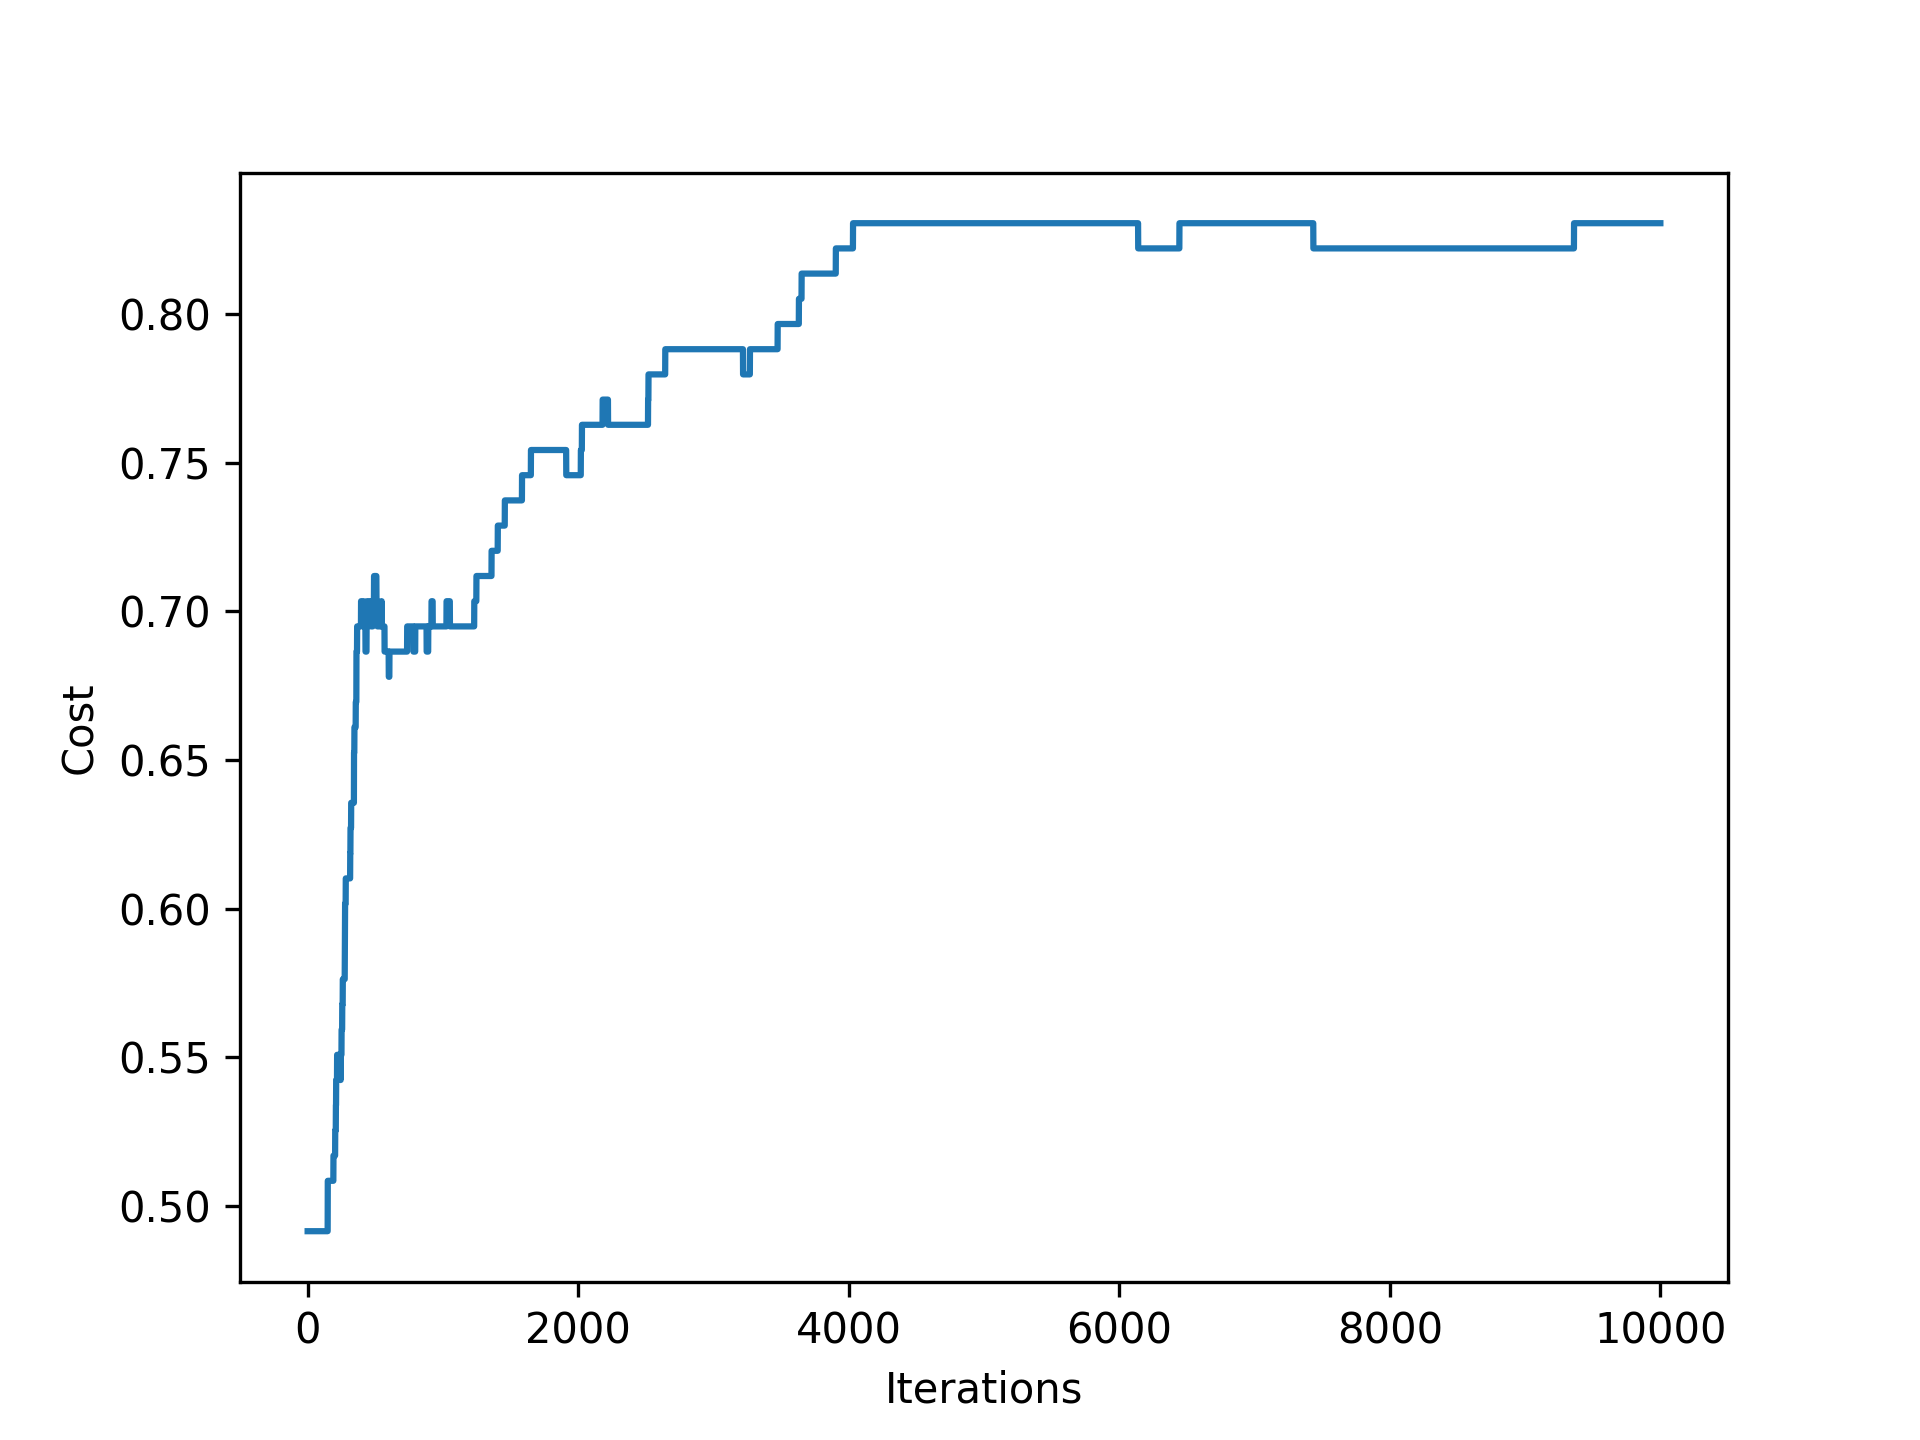
\includegraphics[width=0.5\textwidth]{./imagenes/muestreo2_accuracy.png}
    \caption{Evolución de la predicción para el segundo dataset}
    \label{fig:prediction_evolution2}
\end{figure}

\begin{figure}[H]
    \centering
    \lstinputlisting[firstline=196,lastline=213, style=custompython]{../logistic_reg.py}
    \caption{Función de predicción}
    \label{fig:predict}
\end{figure}

\begin{figure}[H]
    \centering
    \lstinputlisting[firstline=216,lastline=229, style=custompython]{../logistic_reg.py}
    \caption{Función de comprobación de predicción}
    \label{fig:predict_check}
\end{figure}

\begin{figure}[H]
    \centering
    \lstinputlisting[firstline=232,lastline=244, style=custompython]{../logistic_reg.py}
    \caption{Función de carga de datos}
    \label{fig:load_data}
\end{figure}

\begin{figure}[H]
    \centering
    \lstinputlisting[firstline=304,lastline=321, style=custompython]{../logistic_reg.py}
    \caption{Función de ejecución de modelo de estudiantes}
    \label{fig:run_student_sim}
\end{figure}

\begin{figure}[H]
    \centering
    \lstinputlisting[firstline=324,lastline=342, style=custompython]{../logistic_reg.py}
    \caption{Función de ejecución de modelo de chips}
    \label{fig:run_chip_sim}
\end{figure}

\begin{figure}[H]
    \centering
    \lstinputlisting[firstline=287,lastline=301, style=custompython]{../logistic_reg.py}
    \caption{Función de ejecución de pruebas}
    \label{fig:run_tests}
\end{figure}

\begin{figure}[H]
    \centering
    \lstinputlisting[firstline=247,lastline=268, style=custompython]{../logistic_reg.py}
    \caption{Función de visualización de datos de ejemplo}
    \label{fig:plot_ex_data}
\end{figure}

\begin{figure}[H]
    \centering
    \lstinputlisting[firstline=270,lastline=284, style=custompython]{../logistic_reg.py}
    \caption{Función de visualización de datos de evolución de coste y predicción}
    \label{fig:plot_linear_data}
\end{figure}
\end{document}
